% results.tex — Full proposal draft, Week 8
% Updated statistics: N=28, 56 significant ROIs, median r=0.160, ISFC r=0.617.
% Network breakdown updated: DAN 11/14, VAN 14/24, CONT 12/26, DMN 6/26.

\section{Results}

\subsection{Preliminary Results: Movie-Watching Training Phase}

The aPCR pipeline has been run end-to-end on the NNW movie-watching data with N\,=\,28 fNIRS participants paired against all 59 fMRI participants. Three complementary metrics characterize model performance: (1) per-ROI prediction accuracy, assessed by the Pearson correlation between predicted and observed group-mean fMRI; (2) network-level breakdown of significant ROIs; and (3) preservation of large-scale connectivity structure, assessed via inter-subject functional connectivity (ISFC). Significance is assessed throughout with phase-randomization permutation tests (1,000 iterations) and FDR correction (Benjamini-Hochberg, $q < 0.05$) across all 122 ROIs.

\subsubsection{Per-ROI Prediction Accuracy}

Of 122 brain regions, 56 are significantly predicted by the model (FDR $q < 0.05$), with a median Pearson $r = 0.160$ across all ROIs. Figure~\ref{fig:brainmap} shows the spatial distribution of prediction accuracy on the cortical surface. Significant prediction in lateral prefrontal and parietal regions confirms that the model captures real cortical signal in the dorsal attention network (DAN) and frontoparietal control network (CONT), the systems most directly recruited by n-back and CPT tasks \citep{owen2005, cole2013}. Stronger performance in visual and auditory regions is expected given the movie-watching context, as those regions show the most stimulus-consistent responses the model can learn to track.

One finding is noteworthy: visual (VIS) and somatomotor (SM) cortex each reach significance despite the fNIRS cap having no channels over either region. The model has no direct measurement of those areas; it can only reconstruct them through the temporal covariation structure it learned from the regions it does cover. This suggests the model is capturing shared large-scale dynamics rather than purely local signal, consistent with the ISC literature on distributed network responses during naturalistic viewing \citep{hasson2010}. It also warrants caution: prediction of uncovered regions rests on learned statistical relationships, not spatial fidelity, and those relationships may not hold when the temporal context changes from movie-watching to structured tasks.

\begin{figure}[ht]
    \centering
    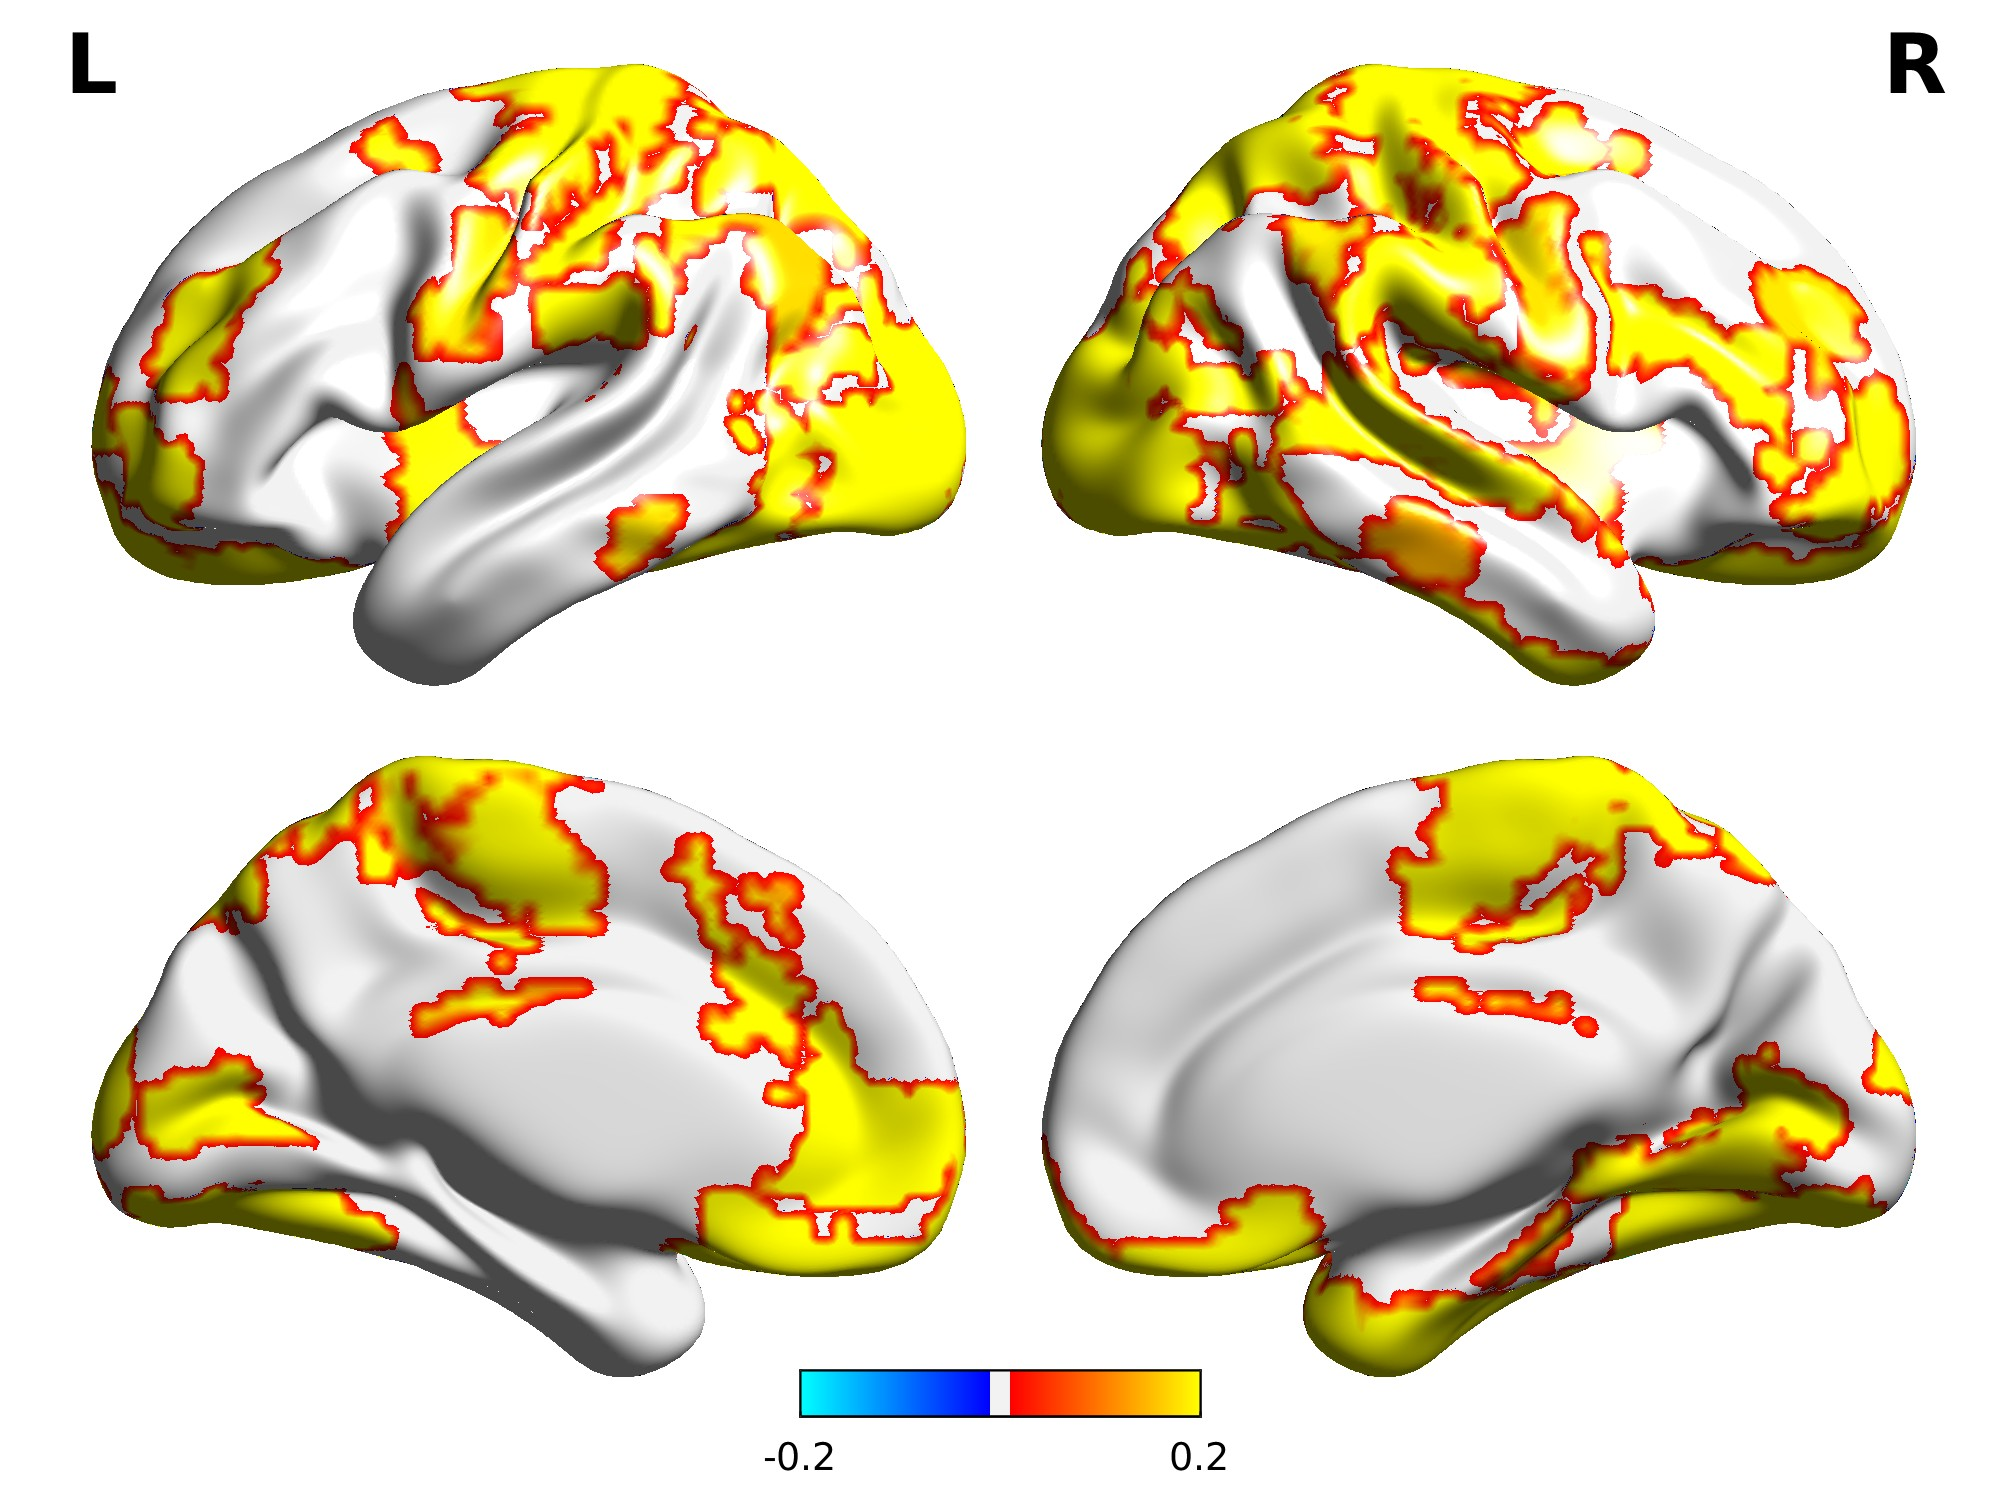
\includegraphics[width=0.85\textwidth]{figures/fig3a_grp_grp_r_pmasked.jpg}
    \caption{Brain surface map of aPCR prediction accuracy (group-level Pearson $r$, FDR-corrected significant ROIs highlighted). Brighter regions indicate ROIs where the model's predicted fMRI time series most closely tracks the observed fMRI. Of 122 ROIs, 56 are significantly predicted (FDR $q < 0.05$), with a median Pearson $r = 0.160$ across all ROIs.}
    \label{fig:brainmap}
\end{figure}

\subsubsection{Network-Level Breakdown}

Figure~\ref{fig:network} shows prediction accuracy broken down by functional network. The dorsal attention network (DAN) shows the strongest proportional performance: 11 of 14 ROIs are significantly predicted (79\%), the highest hit rate of any network. The ventral attention network (VAN) achieves 14 of 24 significant ROIs (58\%). The frontoparietal control network (CONT) reaches 12 of 26 (46\%), and the DMN reaches 6 of 26 (23\%). DAN's dominance is directly relevant to the individual differences hypothesis: DAN is the primary recruitment target of both n-back and CPT tasks \citep{owen2005}, and its strong performance in the training phase supports the expectation that the frozen model will capture task-evoked attention network dynamics.

The CONT performance is particularly encouraging given that this is a large, distributed network with 26 ROIs spread across medial and lateral surfaces, many of which are far from the fNIRS channels. That 12 ROIs survive FDR correction suggests the model is recovering network-level dynamics through temporal covariation rather than purely through direct cortical coverage. DMN performance (6/26) is lower than DAN and CONT, which may reflect reduced DMN engagement during movie-watching relative to resting state, or the fact that medial default-mode nodes are farther from the prefrontal-parietal fNIRS cap. Whether the DMN prediction holds up in task contexts, where DMN suppression is the theoretically predicted signal, is the central open question.

\begin{figure}[ht]
    \centering
    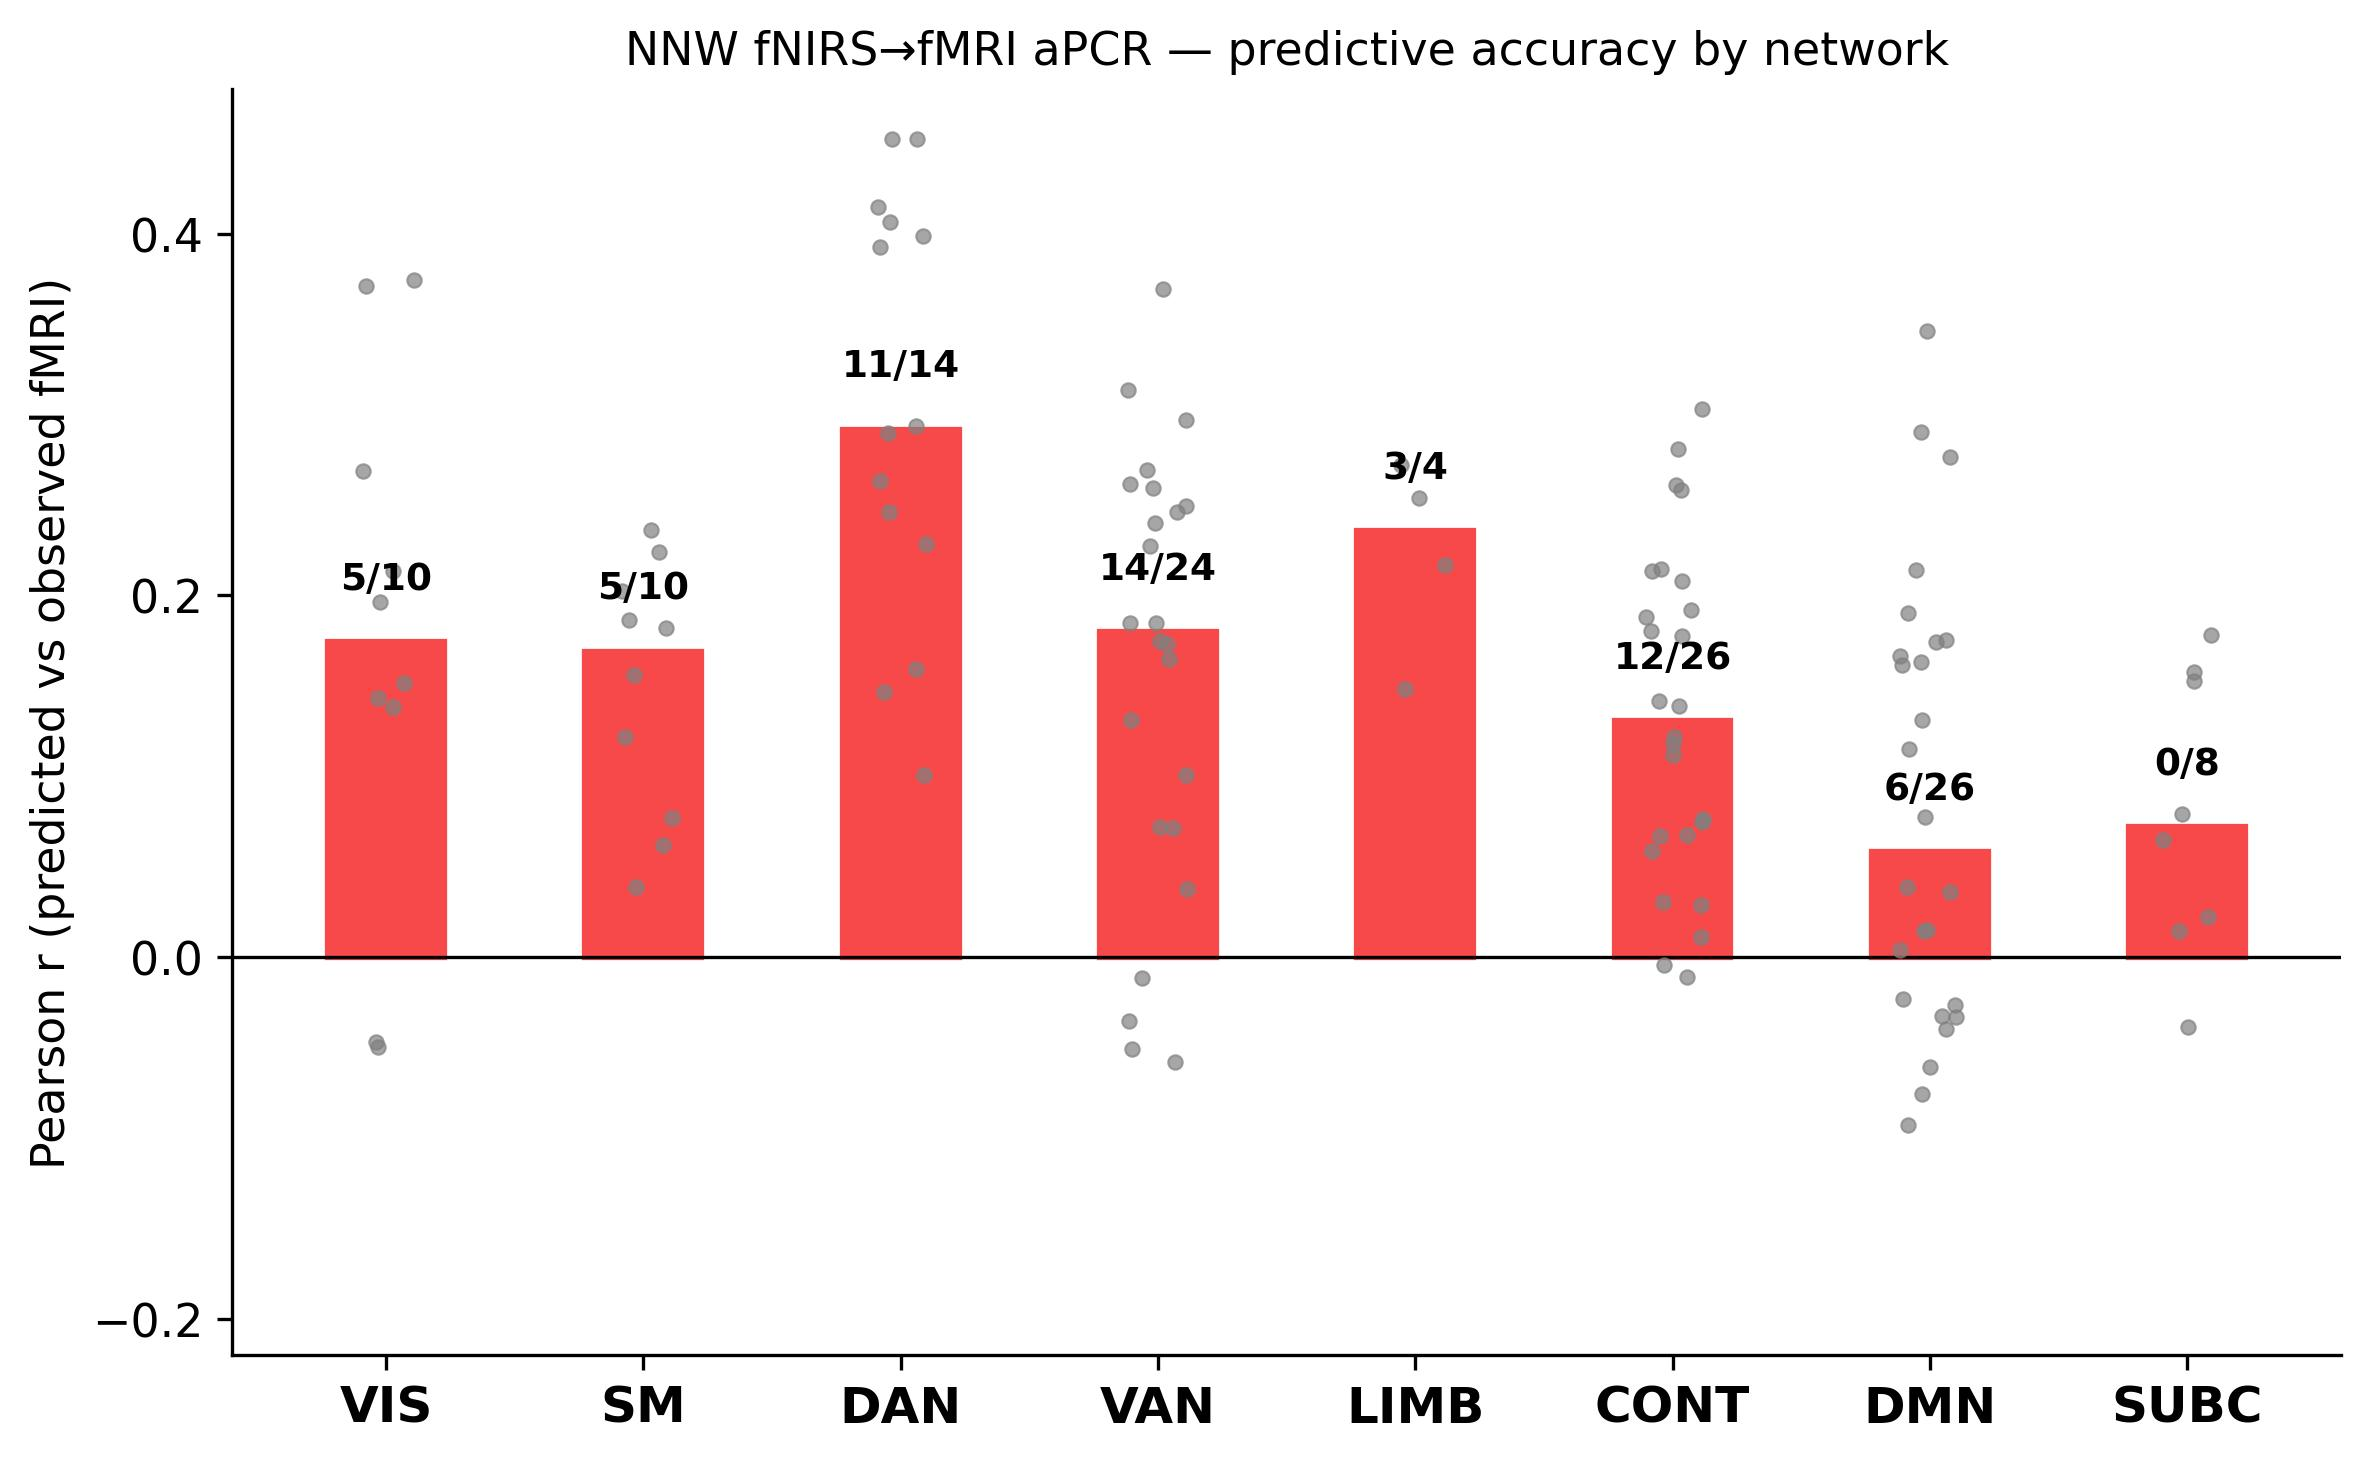
\includegraphics[width=0.85\textwidth]{figures/fig3b_network_barplot.jpg}
    \caption{aPCR prediction accuracy by functional network (Yeo 17-network + Brainnetome + subcortical atlas, collapsed to 8 systems). Bars show median Pearson $r$ across ROIs in each network; overlaid dots show individual ROI values. Fractions indicate the number of significantly predicted ROIs out of the total in each network (FDR $q < 0.05$): DAN 11/14, VAN 14/24, CONT 12/26, DMN 6/26, SM 5/10, VIS 5/10, LIMB 3/4, SUBC 0/8. Networks are ordered from posterior sensory to anterior/higher-order.}
    \label{fig:network}
\end{figure}

\subsubsection{Connectivity Structure Preservation}

The ISFC comparison addresses a question that per-ROI accuracy cannot: does the model preserve the large-scale organizational logic of the brain, not just isolated activation levels? Individual differences in attention are encoded in how networks communicate with one another, specifically in the dynamic balance between frontoparietal task-positive systems and the DMN \citep{cole2013, braun2015}. The Pearson correlation between the observed and predicted ISFC matrices (lower triangles) is $r = 0.617$ ($p = 0.001$, permutation test; Figure~\ref{fig:isfc}). The model is not just predicting individual regions; it is preserving the large-scale organization of how brain regions communicate during the movie. Both matrices show the expected anti-correlation between task-positive networks (DAN, VAN, CONT) and DMN, indicating the model captures the fundamental antagonistic relationship between these systems. This $r = 0.617$ value serves as the NNW benchmark against which cognitive task predictions will be compared.

\begin{figure}[ht]
    \centering
    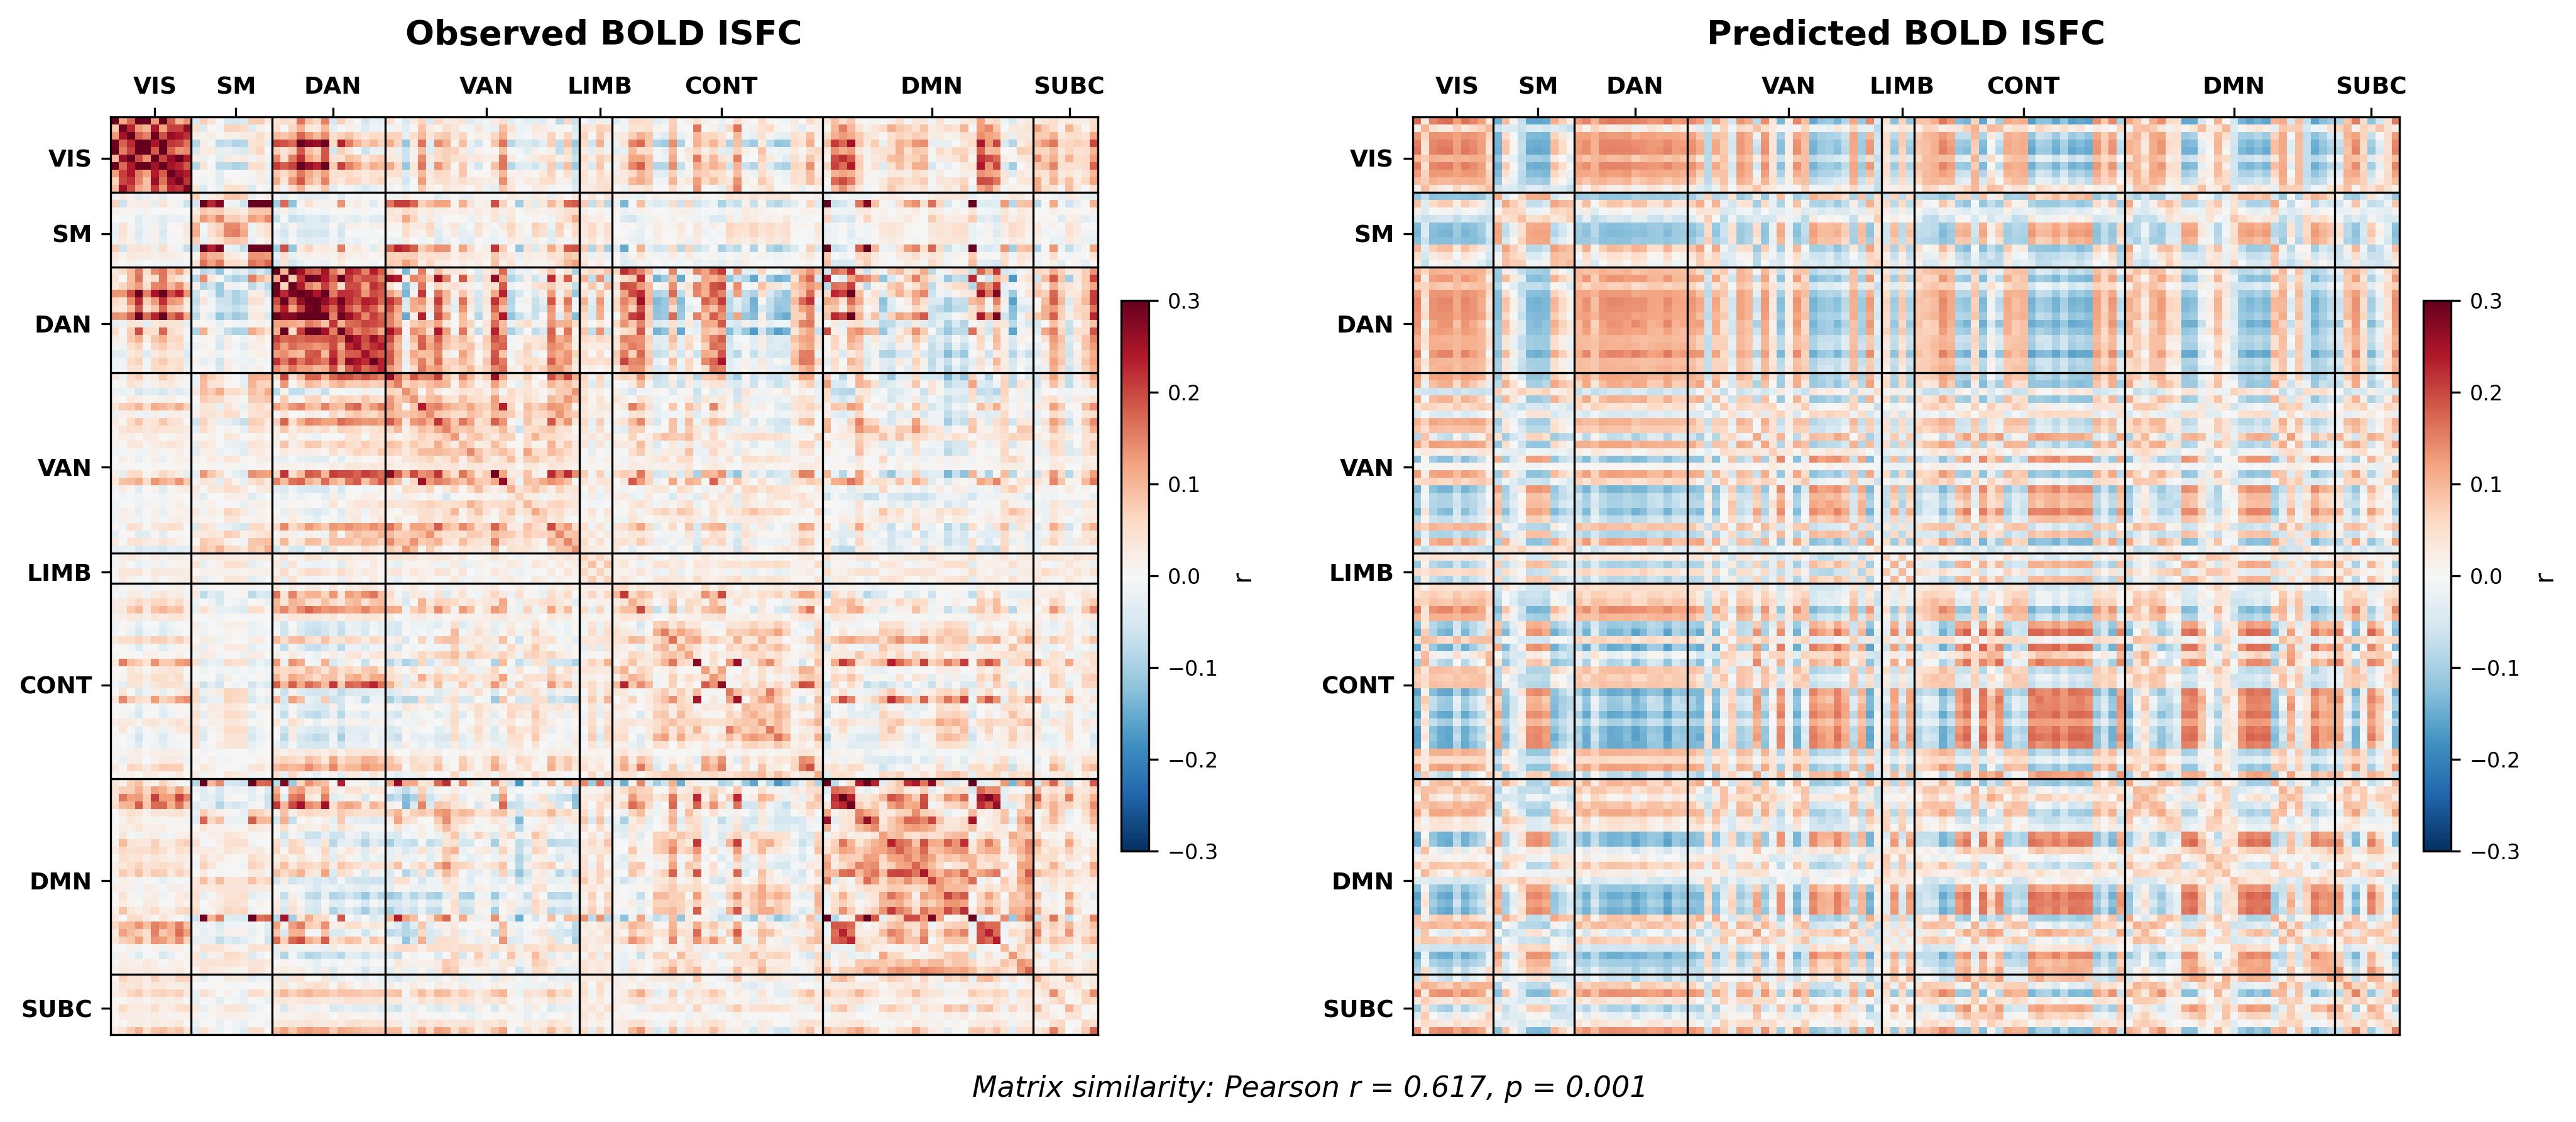
\includegraphics[width=\textwidth]{figures/fig4_isfc_heatmap.jpg}
    \caption{Observed versus predicted BOLD inter-subject functional connectivity (ISFC) matrices. Left: true fMRI ISFC. Right: ISFC reconstructed by the aPCR model from fNIRS signals alone. Each cell represents the average correlation between one ROI's time series and the leave-one-out group mean of another ROI, capturing how brain regions coordinate during the film. The Pearson correlation between the lower triangles of the two matrices is $r = 0.617$ ($p = 0.001$, permutation test).}
    \label{fig:isfc}
\end{figure}

\subsubsection{Independent Replication}

Applying the identical aPCR pipeline to a separate fNIRS dataset collected by a previous lab member (different participants, same NNW clip, same cognitive tasks) yielded 28 significantly predicted ROIs and an ISFC matrix similarity of $r = 0.297$ ($p = 0.001$). Both the number of significant ROIs and the ISFC similarity are lower than the primary dataset, likely reflecting differences in sample size and data quality. However, the result confirms the pipeline is not overfit to a single dataset.

An informative contrast emerges in the network-level pattern. In the replication dataset, the network ranking closely matches \citet{gao2025}: DMN and CONT lead in prediction accuracy. This differs from the primary dataset, where DAN dominates (11/14, 79\%) and CONT and DMN perform well but do not lead. One candidate explanation is task ordering: in the primary dataset, participants watched the movie at the end of a two-hour session after completing all cognitive tasks, whereas the replication dataset used a different session structure. If fatigue or reduced engagement selectively dampens narrative-driven DMN responses while leaving stimulus-driven visual responses intact, this could shift which networks the model predicts most accurately. Future data collection will place the movie-watching block first and include self-report measures of engagement and cap discomfort to test this possibility directly. Regardless of the mechanism, the fact that both datasets produce significant whole-brain predictions through different network emphases suggests the aPCR framework is robust, even if the specific network profile depends on recording conditions.


\subsection{Expected Results: Cross-Task Predictions and Individual Differences}

The preliminary results establish that the aPCR model captures real, network-level brain structure during movie-watching. The following analyses apply the frozen NNW model to cognitive task data and test whether the predictions carry behavioral meaning. These analyses are planned; the specific predictions below are grounded in the existing literature and in the pattern of results from the training phase.

\subsubsection{Expected Result 1: Cross-Task Neural Plausibility}

When the frozen NNW model is applied to n-back fNIRS data, the predicted fMRI time series should show task-appropriate activation patterns even though the model has never encountered structured cognitive tasks. Three specific predictions follow from the fMRI literature on working memory:

First, predicted activation in DAN and CONT ROIs should be higher during 2-back blocks than during 1-back blocks. The n-back task is the most extensively studied working memory paradigm in fMRI, and the meta-analysis by \citet{owen2005} identifies bilateral dorsolateral prefrontal cortex, premotor cortex, and posterior parietal cortex (all within DAN and CONT) as the regions most consistently recruited by increasing working memory load. If the frozen model captures generalizable cortical-subcortical relationships, the predicted activation in these regions should track load even without any task-specific training.

Second, predicted DMN activation should show the inverse pattern: lower activation during 2-back than during 1-back. DMN suppression during cognitively demanding tasks is one of the most replicated findings in the fMRI literature \citep{sonugabarke2007}, and the degree of suppression scales with task difficulty. The model's ability to predict this pattern from surface fNIRS signals would provide strong evidence that the learned mapping captures the antagonistic relationship between task-positive and task-negative systems.

Third, ISFC computed on the predicted cognitive-task fMRI should be lower than the NNW benchmark ($r = 0.617$) but significantly above chance. ISC values near zero are expected for trial-based, non-naturalistic paradigms because individual differences in strategy, arousal, and performance make neural responses less consistent across participants \citep{nastase2019}. A meaningful but attenuated ISFC would indicate that the model is capturing whatever shared structure exists in the task data rather than producing noise.

I will quantify these patterns using paired $t$-tests comparing predicted ROI activation between 1-back and 2-back blocks, computed separately for each functional network. Effect sizes (Cohen's $d$) will be reported alongside significance to characterize the magnitude of any load-dependent differences the model detects.

\subsubsection{Expected Result 2: Behavioral Correlates of Predicted Neural Patterns}

The central individual-differences hypothesis is that predicted brain patterns should correlate with how well participants actually perform the cognitive tasks. The analyses are organized around three behavioral measures: reaction time variability, task accuracy, and signal detection sensitivity.

\paragraph{Reaction time variability and DMN dynamics.} The most theoretically grounded prediction concerns the relationship between predicted DMN activation and reaction time variability (RTV). RTV is computed as the intraindividual standard deviation of correct-trial reaction times (iSD-RT) within each participant for each task and load condition. During goal-directed tasks, the DMN is normally suppressed; when suppression fails periodically, the DMN reactivates and disrupts processing, producing attentional lapses that manifest as unusually slow, variable responses \citep{sonugabarke2007, kofler2013}. The prediction is directional: participants with higher predicted DMN mean activation during the n-back should show higher RTV (Figure~\ref{fig:dmn_rtv}).

I will test this with Pearson correlations between per-subject predicted DMN mean activation (averaged across the 26 DMN ROIs and across task blocks) and per-subject iSD-RT, computed separately for 1-back and 2-back conditions. The expected effect size is $r \approx 0.35$ to $0.45$, attenuated from published fMRI-behavior correlations ($r \approx 0.50$ to $0.60$; \citealp{braun2015, finn2021}) to account for the information loss inherent in model-predicted rather than directly measured fMRI. At the current sample size (N\,=\,28), effects in the $r \approx 0.40$ range are detectable but underpowered for stringent correction. The project targets N\,=\,40, at which effects of this magnitude achieve approximately 80\% power.

The same analysis will be run using the coefficient of variation of RT (CV-RT\,=\,SD/Mean) as an alternative operationalization of RTV. CV-RT controls for differences in mean RT across participants, which matters if some participants adopt a generally slower response strategy rather than experiencing genuine attentional lapses. If both iSD-RT and CV-RT correlate with predicted DMN activation in the same direction, this strengthens the interpretation that the model is capturing DMN-mediated attentional instability rather than overall response speed.

\begin{figure}[ht]
    \centering
    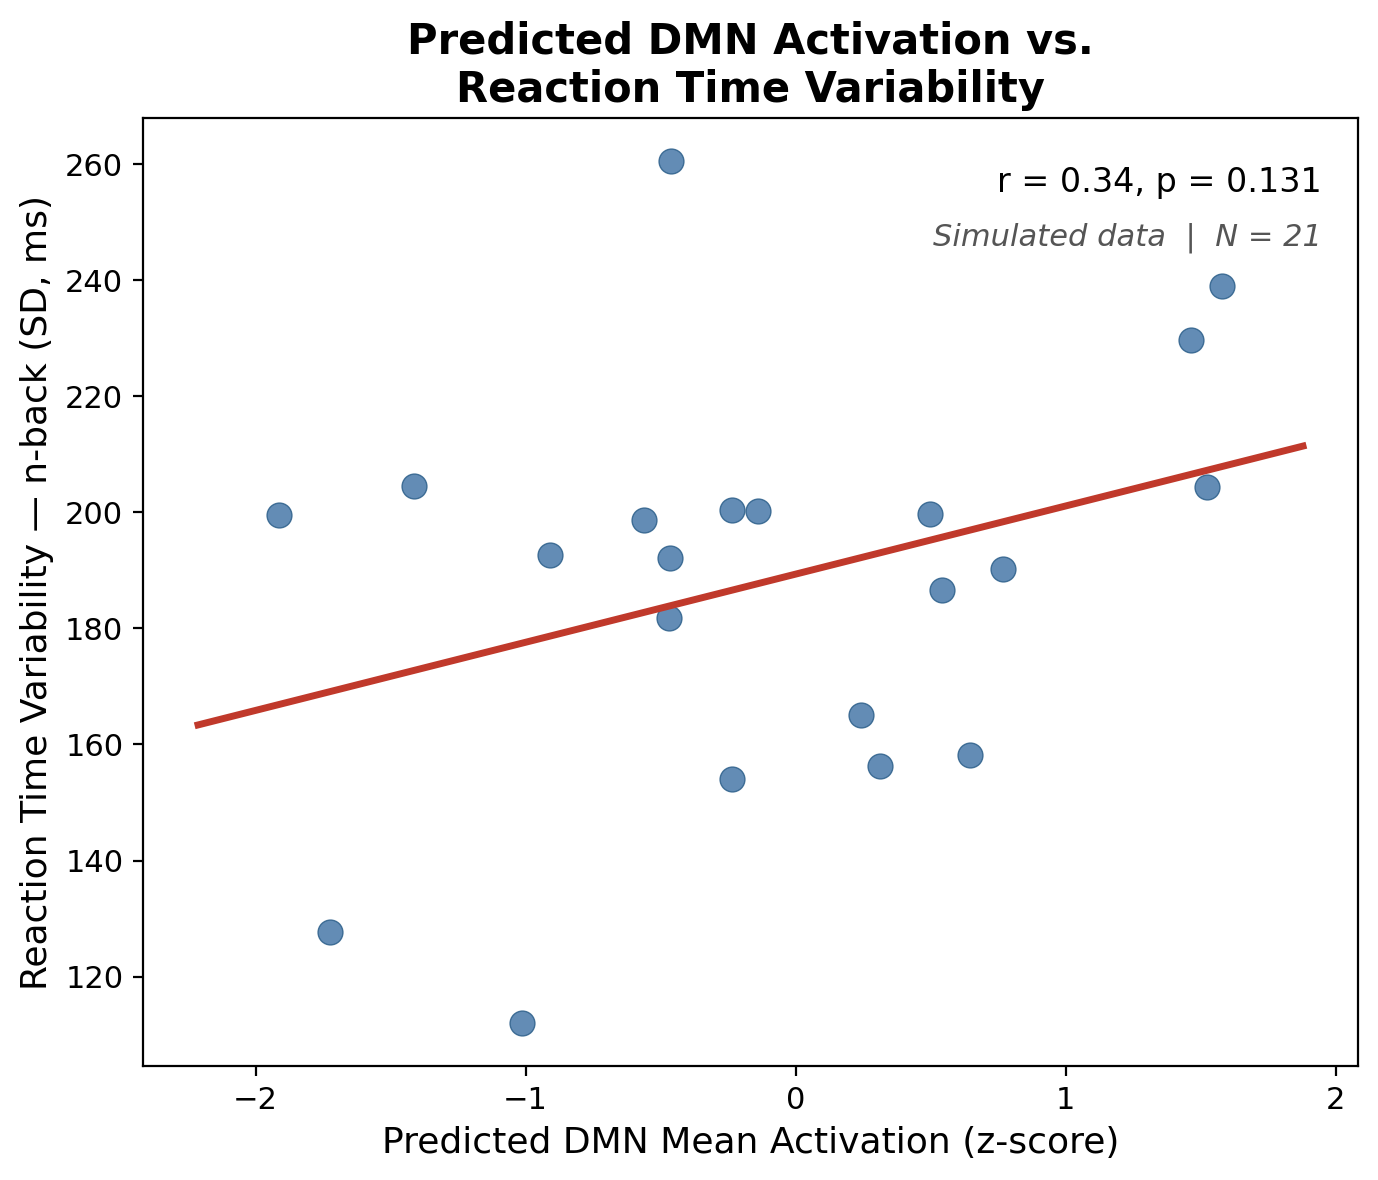
\includegraphics[width=0.65\textwidth]{figures/fig_mockup_dmn_rtv.png}
    \caption{Simulated data. Expected relationship between predicted DMN mean activation during the n-back task and reaction time variability (SD of response times across trials). Data were simulated for N\,=\,28 participants using a target correlation of $r = 0.40$, consistent with the hypothesis that greater DMN intrusion during task performance is associated with more variable response times. Predicted DMN activation was drawn from a standard normal distribution; RTV was generated as a linear combination of DMN activation and independent noise, scaled to realistic n-back RT distributions (mean SD $\approx$ 200\,ms, range $\approx$ 120--280\,ms). This figure illustrates the expected direction and approximate magnitude of the effect; actual values will depend on cognitive task preprocessing results.}
    \label{fig:dmn_rtv}
\end{figure}

\paragraph{Task accuracy and frontoparietal engagement.} Beyond RTV, I will test whether predicted DAN and CONT mean activation during n-back blocks correlates with n-back accuracy (proportion correct, computed separately for 1-back and 2-back). The literature predicts positive correlations: participants whose frontoparietal networks show greater task-evoked reconfiguration tend to perform better on working memory tasks \citep{braun2015, cole2013}. The expected effect size is smaller than the DMN-RTV relationship ($r \approx 0.25$ to $0.35$), and ceiling effects in 1-back accuracy (where most healthy young adults score near-perfect) may limit the sensitivity of this analysis in the 1-back condition. The 2-back condition, which produces more variance in accuracy, is the stronger test.

\paragraph{CPT signal detection and sustained attention.} For the CPT, I will compute d-prime and criterion from hit and false alarm rates (with a 0.5-trial correction for boundary cases) and correlate these with predicted mean activation in DAN and CONT. RTV from the CPT will also be computed and correlated with predicted DMN activation, replicating the n-back analysis in a sustained attention context. Consistent DMN-RTV correlations across both n-back and CPT would strengthen the case that the model captures a domain-general attentional stability mechanism rather than task-specific variance.

\subsubsection{Expected Result 3: Load-Dependent Prediction Quality}

Comparing prediction quality across conditions that differ in cognitive load will reveal whether the naturalistic mapping captures dynamics that scale with task demands. Specifically, I will compute per-ROI prediction variance explained ($R^2$) separately for 1-back and 2-back blocks and compare them using paired $t$-tests across the 56 significant NNW ROIs. Two outcomes are possible, and each is informative:

If prediction quality is comparable across load levels, this suggests the NNW-trained mapping captures a stable cortical-subcortical relationship that persists regardless of cognitive demand, supporting the case for naturalistic calibration as a universal tool. If prediction quality degrades with increasing load, this would indicate that the mapping captures baseline and low-demand dynamics better than executive-control dynamics, establishing a meaningful boundary condition on the approach. Either result advances the field's understanding of when and where naturalistic calibration works.

\subsubsection{Summary of Planned Statistical Tests}

Table~\ref{tab:tests} summarizes the planned analyses, specifying the predictor, outcome, and expected direction for each test.

\begin{table}[ht]
\centering
\small
\caption{Planned individual-differences analyses. All correlations are Pearson $r$, computed across subjects separately for each task and condition. FDR correction is applied across tests within each family.}
\label{tab:tests}
\begin{tabular}{p{3.5cm} p{3.5cm} p{2.5cm} p{2.5cm}}
\hline
\textbf{Neural predictor} & \textbf{Behavioral outcome} & \textbf{Expected direction} & \textbf{Task/condition} \\
\hline
Predicted DMN mean activation & iSD-RT (RTV) & Positive ($r \approx 0.40$) & n-back 1B, 2B \\
Predicted DMN mean activation & CV-RT & Positive & n-back 1B, 2B \\
Predicted DAN mean activation & Accuracy (\% correct) & Positive ($r \approx 0.30$) & n-back 2B \\
Predicted CONT mean activation & Accuracy (\% correct) & Positive & n-back 2B \\
Predicted DAN mean activation & d-prime & Positive & CPT \\
Predicted DMN mean activation & iSD-RT (RTV) & Positive & CPT \\
2B--1B predicted DAN contrast & 2B--1B accuracy change & Positive & n-back \\
\hline
\end{tabular}
\end{table}
